\chapter{RESULTADOS E DISCUSSÕES}
\label{chap:proposta_experimental}

Este capítulo traz informações relacionadas com as ferramentas utilizadas no experimento, como linguagem, bibliotecas utilizadas, entre outros. Assim como, informações sobre o consumo de dados das bases \gls{ACDC} e SunnyBrook, fase de pré-processamento, inferência nos modelos implementados, sendo estes, modelo linha de base e derivados, e modelos adaptados. Por fim, são apresentados os resultados considerando as métricas apresentadas na seção \ref{subsec:cap4_metrics} utilizando as bases de dados ACDC e SunnyBrook e cada uma das abordagens: o modelo base e o modelo proposto.

Por fim, este capítulo apresenta os resultados da prova de conceito realizada com os algoritmos desenvolvidos, tanto o modelo base quanto os modelos adaptados, com o intuito de compará-los aos objetivos traçados nesta dissertação. Os testes realizados buscam avaliar a eficiência do algoritmo sob as diversas adaptações discutidas. 

%--------------------------------------------------------
\section{Materiais} 
\label{sec:cap5_materiais}

A Tabela \ref{tab:hardware_software} apresenta as ferramentas que foram utilizadas nesse projeto. Destaca-se que foram utilizadas majoritariamente ferramentas open-source como a linguagem \textit{python}, bibliotecas como \textit{pyradiomics}, \textit{torch}, \textit{numpy}, entre outras. Para registro dos experimentos, foi utilizada a ferramenta CometML\footnote{https://www.comet.com}. No CometML é possível armazenar valores como: erro do lote no treinamento, acurácia do conjuntos de validação no treinamento, métricas resultantes como acurácia, hiperparâmetros como taxa de aprendizado, épocas, etc.
\newline

\begin{table}[hbtp]
    \caption{Fonte: Componentes Utilizados}
    \centering
    \renewcommand{\arraystretch}{1} % default é 1 
    % \begin{tabular}{|>{\centering\arraybackslash}p{2cm}|p{12cm}|}
    \begin{tabular}{|c|c|}
    \hline 
       \textbf{Item} & \textbf{Descrição}\\
    \hline 
       Computador & \textit{Macbook M1 Pro}  \\
    \hline 
       Memória & 16gb  \\
    \hline 
       Versão \textit{Python} & 3.11.0  \\
    \hline 
       Versão \textit{pyradiomics} & 3.0.1 \\
    \hline 
       Versão \textit{torch} & 2.2.1 \\
    \hline 
       Versão \textit{torchvision} & 0.17.1 \\
    \hline 
       Versão \textit{numpy} & 1.26.4 \\
    \hline 
       Versão \textit{scikit-learn} & 1.4.1.post1 \\
    \hline 
       Versão \textit{comet-ml} & 3.47.4 \\
    \hline 
    \end{tabular} 
    \caption*{Fonte: Autor}
    \label{tab:hardware_software}
\end{table}

%--------------------------------------------------------
\section{Conjunto de Dados} 
\label{subsec:cap5_dataset}

Este trabalho visou realizar os experimentos em duas bases distintas com imagens de \gls{RMC}, informações a cerca do paciente e rótulos que indicam presença ou não de cardiomiopatia. Testes iniciais foram feitos no conjunto de dados \gls{ACDC} que possui $30$ casos de \gls{CMH}, $30$ casos de \gls{CMD} e $90$ casos normais, resultando em $60$ casos de cardiomiopatia e $90$ casos normais. Da base \gls{ACDC} se pretende utilizar apenas as fatias da fase diastólica. O segundo conjunto de dados é o \textit{SunnyBrook}, possuindo imagens na fase diastólica contendo as classes $9$ classes NOR(normal) e $12$ HIP(hipertrofia do ventrículo esquerdo).

O modo de operação será o mesmo para ambos os conjuntos de dados com exceção do pré-processamento dado ao fato da forma como o conjunto de dados \textit{SunnyBrook} disponibiliza as máscaras.

%--------------------------------------------------------
\section{Experimentos Modelo Base}
\label{sec:cap5_experimentos_base}

Uma prova de conceito foi aplicada ao conjunto de dados \gls{ACDC} utilizando o modelo de linha de base para avaliação inicial, avaliação esta também utilizada como linha de base. O modelo base foi implementado seguindo o artigo e sua implementação é conferida na Figura \ref{fig:fig008}. O conjunto de dados para treino é composto por $100$ exames de pacientes, coletando apenas as fatias das imagens da fase diastólica. Características de primeira ordem e \gls{GLCM} são extraídas, utilizando a blbioteca \textit{PyRadiomics}, resultando em $\RadiomicFeatures$ valores que compõem as características radiômicas. Para extração das características profundas, foi utilizado uma rede \textit{ResNet50} congelada sem sua última camada linear, responsável pela classificação originalmente de $1000$ classes oriundas do conjunto de dados \textit{ImageNet}, obtendo como resultado final um vetor com $\DeepFeatures$ características profundas.

% O \textit{F-Test} é utilizado como um seletor de características inicial, aplicado tanto nas características radiômicas quanto nas profundas, reduzindo garantindo que os vetores possuam m profundas, com um total de $\text{EMBED}_{size}$ igual a $12$  no modelo base. As características resultantes do \textit{F-Test}, agora com tamanhos agora iguais, são concatenadas e enviadas ao módulo de autoatenção e os resultados armazenados.

Neste experimento foi treinado o modelo utilizando, como função objetivo a entropia cruzada binária, taxa de aprendizado de $\LR$, otimizador \textit{Adam}, tamanho de lote $\Batch$ e o treinamento se deu com aproximadamente $\Epochs$ épocas, onde verificou que o erro se torna estável em tempo de treinamento. Também foi empregada a estratégia de aleatorizar as entradas no modelo em tempo de treinamento. Ao vetor resultante da saída do modelo é aplicada a função sigmoide, conforme Equação. \ref{eq:sigmoide}, função esta que limita os valores de sua entrada entre 0 e 1. Para fins de classificação, foi considerado valores maiores que $0,5$ são considerados com cardiomiopatia e menores ou iguais a $0,5$ são considerados normais.

\begin{equation}
\textit{sigmoide}(x) = \frac{1}{1 + e^{-x}}
\label{eq:sigmoide}
\end{equation}

% --------------------------------------------------------
\section{Experimentos Modelos Adaptados}
\label{sec:cap5_experimentos_adaptados}

Os modelos adaptados refletem os experimentos desmembrados do modelo base, adaptações estas com a finalidade de verificar se mudanças, seja nos hiperparâmetros, seja em partes da arquitetura, podem trazer resultados promissores em relação aos resultados base. As mudanças podem ser elencadas em: 

\begin{enumerate}

\item Mudanças do $\text{EMBED}_{size}$ onde se foi testado os valores $[24, 48, 64]$ na tentativa de preservar mais informações originais.

\item No caso das versões adaptadas, também há a adição do consumo das respectivas máscaras que são futuramente concatenadas as características radiômicas e profundas.

\item A concatenação é feita de forma diferente, assumindo por exemplo o valor de $\text{EMBED}_{size}$ igual a $12$, na versão original temos como resultado $1\times24$ porém na versão adaptada essa concatenação é feita na primeira dimensão, resultando neste exemplo em $2\times12$. Isto se dá pois é apresentado um novo bloco ao modelo original o bloco convolucional, composto de convolução e blocos \gls{SE}.

\end{enumerate}


A parte restante da arquitetura segue de acordo com a original, exceto que também podemos variar $N$ vezes o bloco de autoatenção, ou seja, sua saída volta sendo sua entrada $N$ vezes e este valor de $N$ também pode ser considerado como um dos hiperparâmetros do experimento. Os valores de $N$ utilizados foram $[1, 2, 4, 6]$. Estas mudanças não mudam a estrutura da arquitetura incial fazendo com que o módulo autoatenção seja executado $N$ vezes conforme trabalho de \cite{vaswaniAttentionAllYou2023} e pode ser visualizada na Figura \ref{fig:fig030}.

\begin{figure}[H]
    \centering
    \caption{Recorrência do Módulo de Autoatenção}
    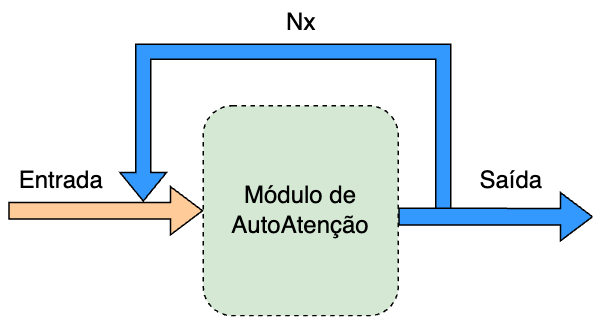
\includegraphics[width=0.7\textwidth]{figures/fig030.png}
    \caption*{Fonte: Autor}
    \label{fig:fig030}
\end{figure}


% Posso elencar novamente de forma sucinta os hiperparamentros aqui: EMBED_SIZE, N attention blocks, imagems de mascara e nova forma de concatenar. 


%--------------------------------------------------------
% \section{Cronograma}
% \label{sec:cronograma}

% O cronograma proposto das atividades segue na Figura \ref{fig:fig014}. Os itens em azul são atividades concluídas como: disciplinas, revisão bibliográfica, refinamento do tema, testes iniciais, etc. Itens em rosa são atividades em andamento como: implementação de modelos de comparação e escrita da dissertação. Atividades em amarelo são atividades planejadas como: análise de resultados, escrita da dissertação e escrita de artigos.

% \begin{figure}[htbp]
%     \centering
%     \caption{Cronograma planejado}
%     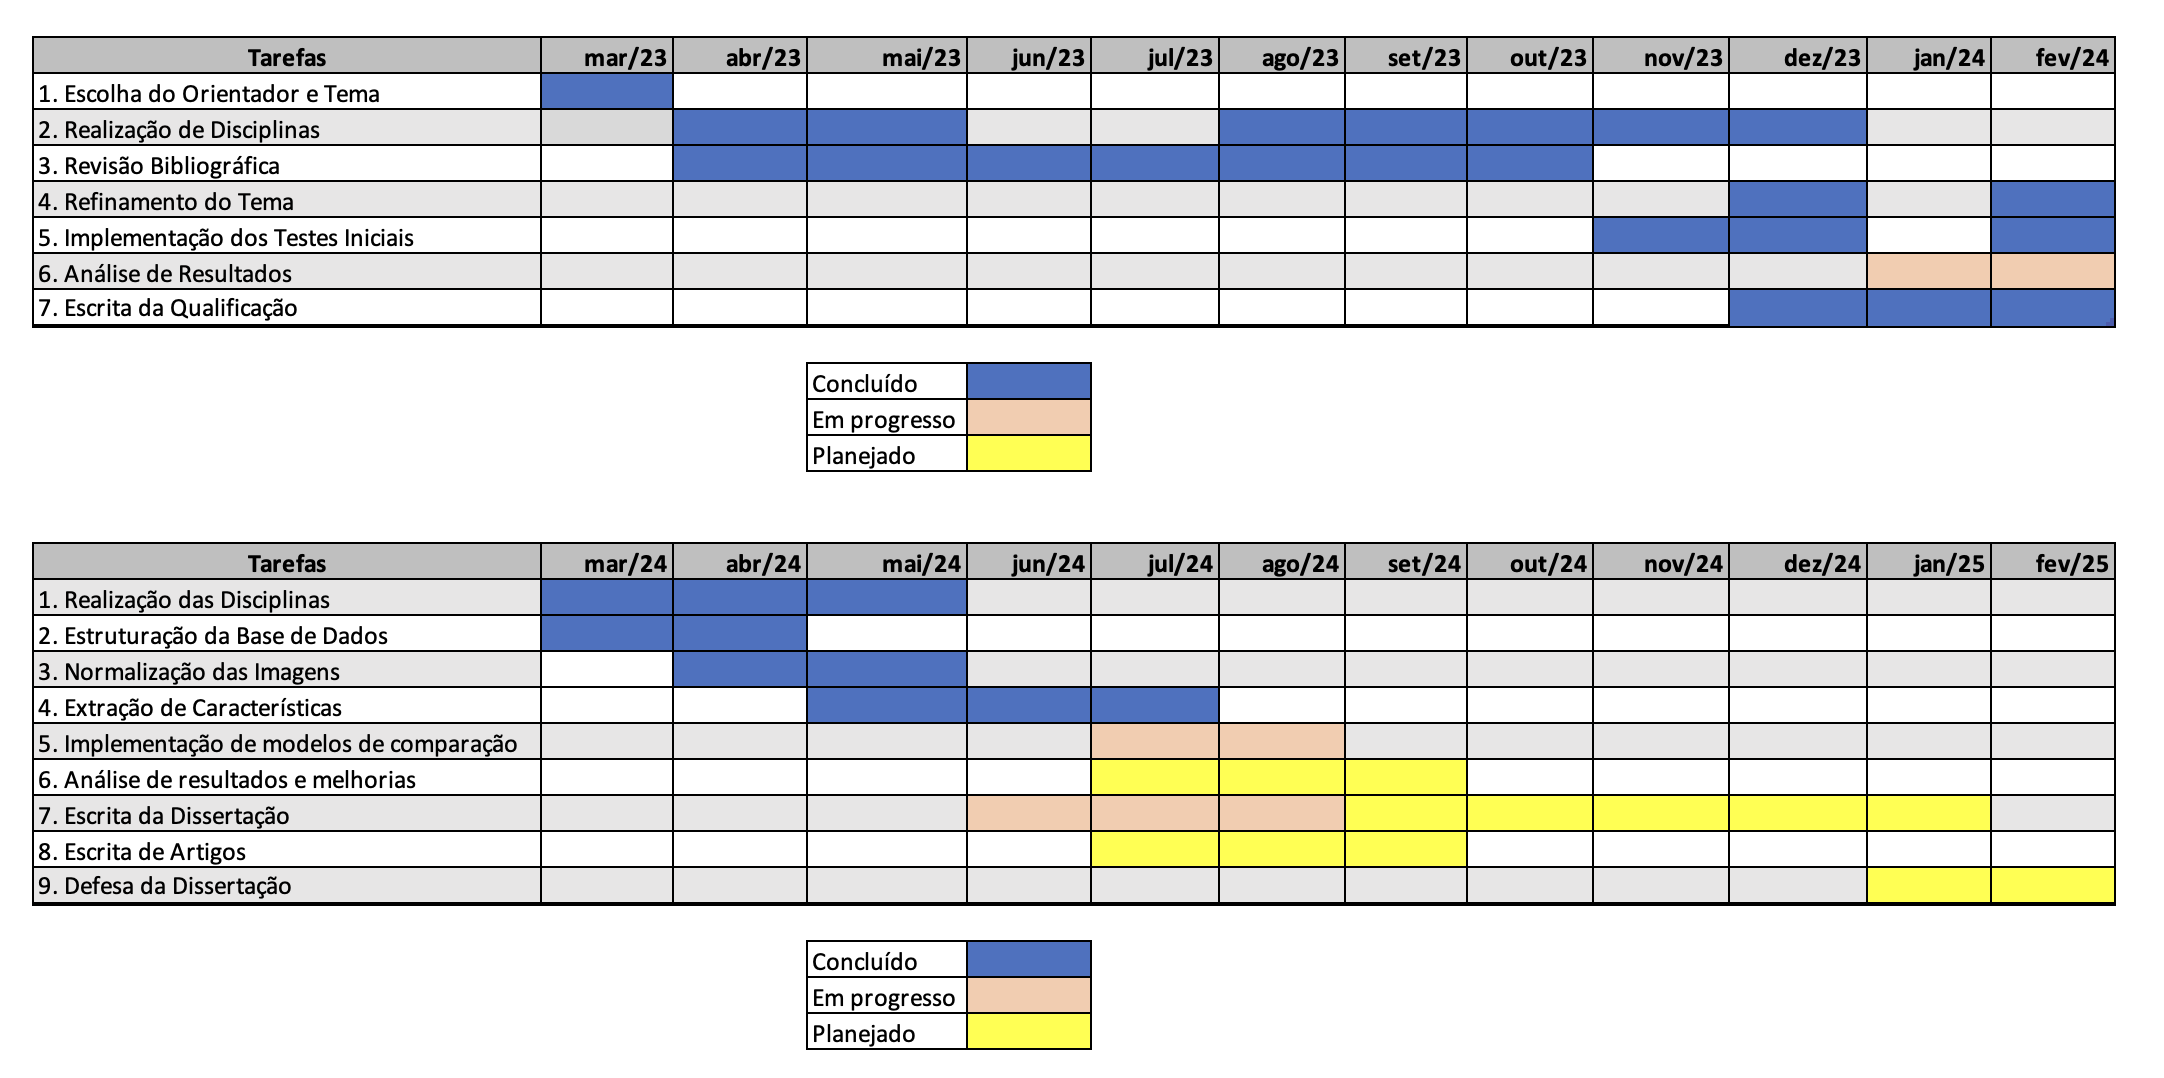
\includegraphics[width=1\textwidth]{figures/fig014.png}
%     \caption*{Fonte: Autor}
%     \label{fig:fig014}
% \end{figure}

%--------------------------------------------------------
\section{RESULTADOS ACDC}
\label{sec:resultados_acdc}

O conjunto de dados \gls{ACDC} foi a referência inicial, principalmente para a coleta dos resultados com o modelo base. Este conjunto de dados público já se encontra separado com $100$ exames para treino e $50$ para testes. A Figura \ref{fig:fig018} e \ref{fig:fig019} são exemplos respectivamente, de imagens de \gls{DCM} e \gls{HCM} capturadas na diástole com suas respectivas máscaras, lembrando que ambas representam cardiomiopatia hipertrófica. Na Figura \ref{fig:fig020} temos a imagem de coração em estado sem anomalia (\gls{NOR}) e sua respectiva máscara. As imagens demonstradas fazem parte do conjunto real de treinamento.

\begin{figure}[h!]
    \centering
    \caption{Captura Diastólica CMD}
    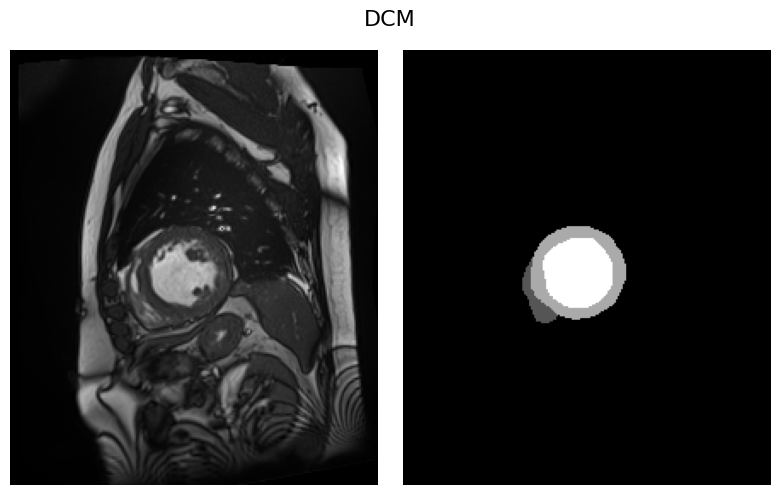
\includegraphics[width=0.65\textwidth]{figures/fig018.png}
    \caption*{Fonte: Autor}
    \label{fig:fig018}
\end{figure}

\begin{figure}[h!]
    \caption{Captura Diastólica de CMH}
    \centering
    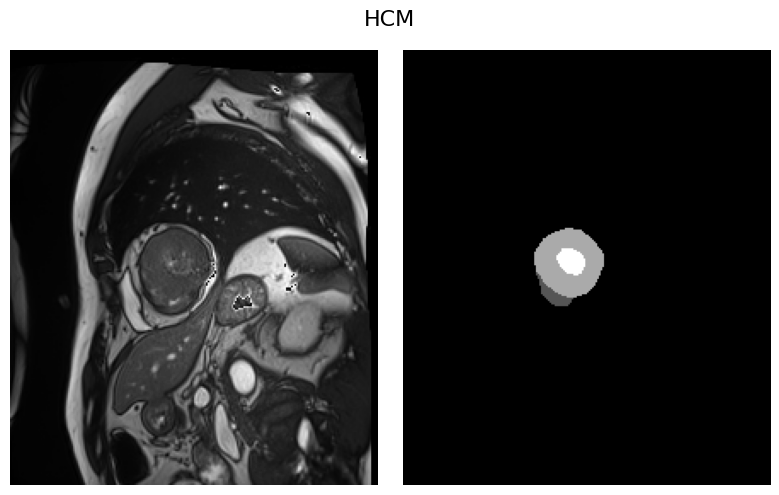
\includegraphics[width=0.65\textwidth]{figures/fig019.png}
    \caption*{Fonte: Autor}
    \label{fig:fig019}
\end{figure}

\begin{figure}[h!]
    \centering
    \caption{Captura Diastólica NOR}
    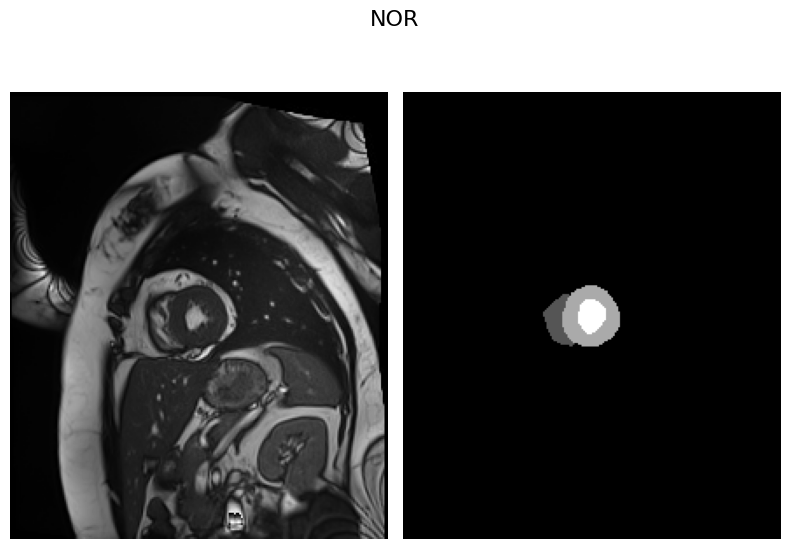
\includegraphics[width=0.65\textwidth]{figures/fig020.png}
    \caption*{Fonte: Autor}
    \label{fig:fig020}
\end{figure}

%--------------------------------------------------------
\subsection{Resultados dos Modelos Base - ACDC}
\label{subsec:resultados_acdc_base}

Com os dados pré-processados e previamente armazenados, o treinamento é efetuado com os vetores radiômicos e profundos. As métricas parciais foram sendo salvas em tempo de treinamento. Para o modelo base os hiperparâmetros são: $\text{EMBED}_{size}$ igual a $12$, $N$ igual 1, ou seja, apenas um bloco de auto atenção, dimensão de concatenação $1$, taxa de aprendizado $\LR$, otimizador \gls{Adam}, tamanho de lote $\Batch$ e aproximadamente $\Epochs$ épocas. Uma vez treinado, foi feita a inferência no conjunto de dados de teste, aplicando a função sigmoide e definindo $0,5$ como o valor de corte onde os valores acima deste limite são classificados como \gls{CMH} e os demais como normal. 

As métricas resultantes podem ser conferidas na Tabela \ref{tab:metrics}. A matriz de confusão é apresentada na Figura \ref{fig:fig016} e um gráfico ilustrando da \gls{ROC} é apresentado na Figura \ref{fig:fig017}.
\newline

\begin{table}[h!]
    \centering
    \caption{Métricas do Experimento - Modelo Base}
    \renewcommand{\arraystretch}{1} % default é 1 
    \begin{tabular}{|c|c|}
    \hline 
          \textbf{Métrica} & \textbf{Valor} \\ 
    \hline 
        Acurácia & 0.58 \\ 
    \hline 
        Precisão & 0.47 \\ 
    \hline 
        Revocação & 0.45 \\ 
    \hline 
        AUC & 0.55 \\ 
    \hline 
    \end{tabular} 
    \caption*{Fonte: Autor}
    \label{tab:metrics}
\end{table}

\begin{figure}[h!]
    \centering
    \caption{Matriz de Confusão -  Modelo Base}
    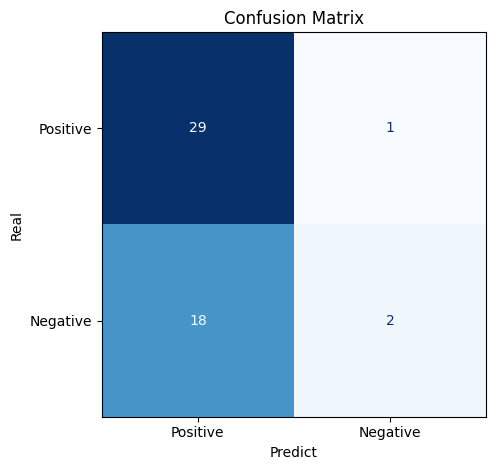
\includegraphics[width=0.55\textwidth]{figures/fig016.png}
    \caption*{Fonte: Autor}
    \label{fig:fig016}
\end{figure}

\begin{figure}[h!]
    \centering
    \caption{ROC}
    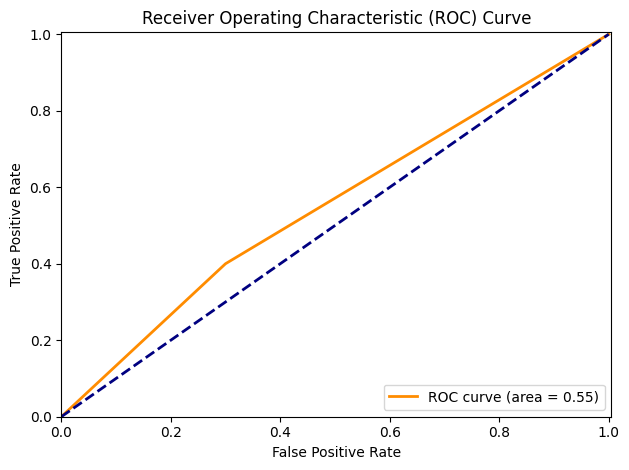
\includegraphics[width=0.75\textwidth]{figures/fig017.png}
    \caption*{Fonte: Autor}
    \label{fig:fig017}
\end{figure}


Para o registro dos resultados foi utilizado a ferramenta \textit{CometML}. O \textit{CometML} pode registrar, em tempo de execução, informações como erro por lote, erro por época, acurácia de validação, etc, podem ser armazenados enquanto o processo de treinamento é executado. Por fim métricas como acurácia e matriz de confusão podem ser armazenadas também. O serviço é acessado  por uma \gls{API} externa. As Figuras \ref{fig:fig028} e \ref{fig:fig029} demonstram respectivamente os painéis adaptáveis com alguns dos hiperparâmetros e métricas coletadas durante e ao terminar o treino. É possível notar que o modelo se sobre-ajusta nos dados de treino, acom acurácia $1$, predizendo corretamente todos os valores porém, nos dados de teste a assertividade cai drasticamente para $0,58$. Também é possível notar que após $2500$ passos no treinamento, o erro de treinamento estabiliza e os demais processamentos não se fazem necessários.

\begin{figure}[h!]
    \centering
    \caption{Painéis Adaptáveis - \textit{CometML}}
    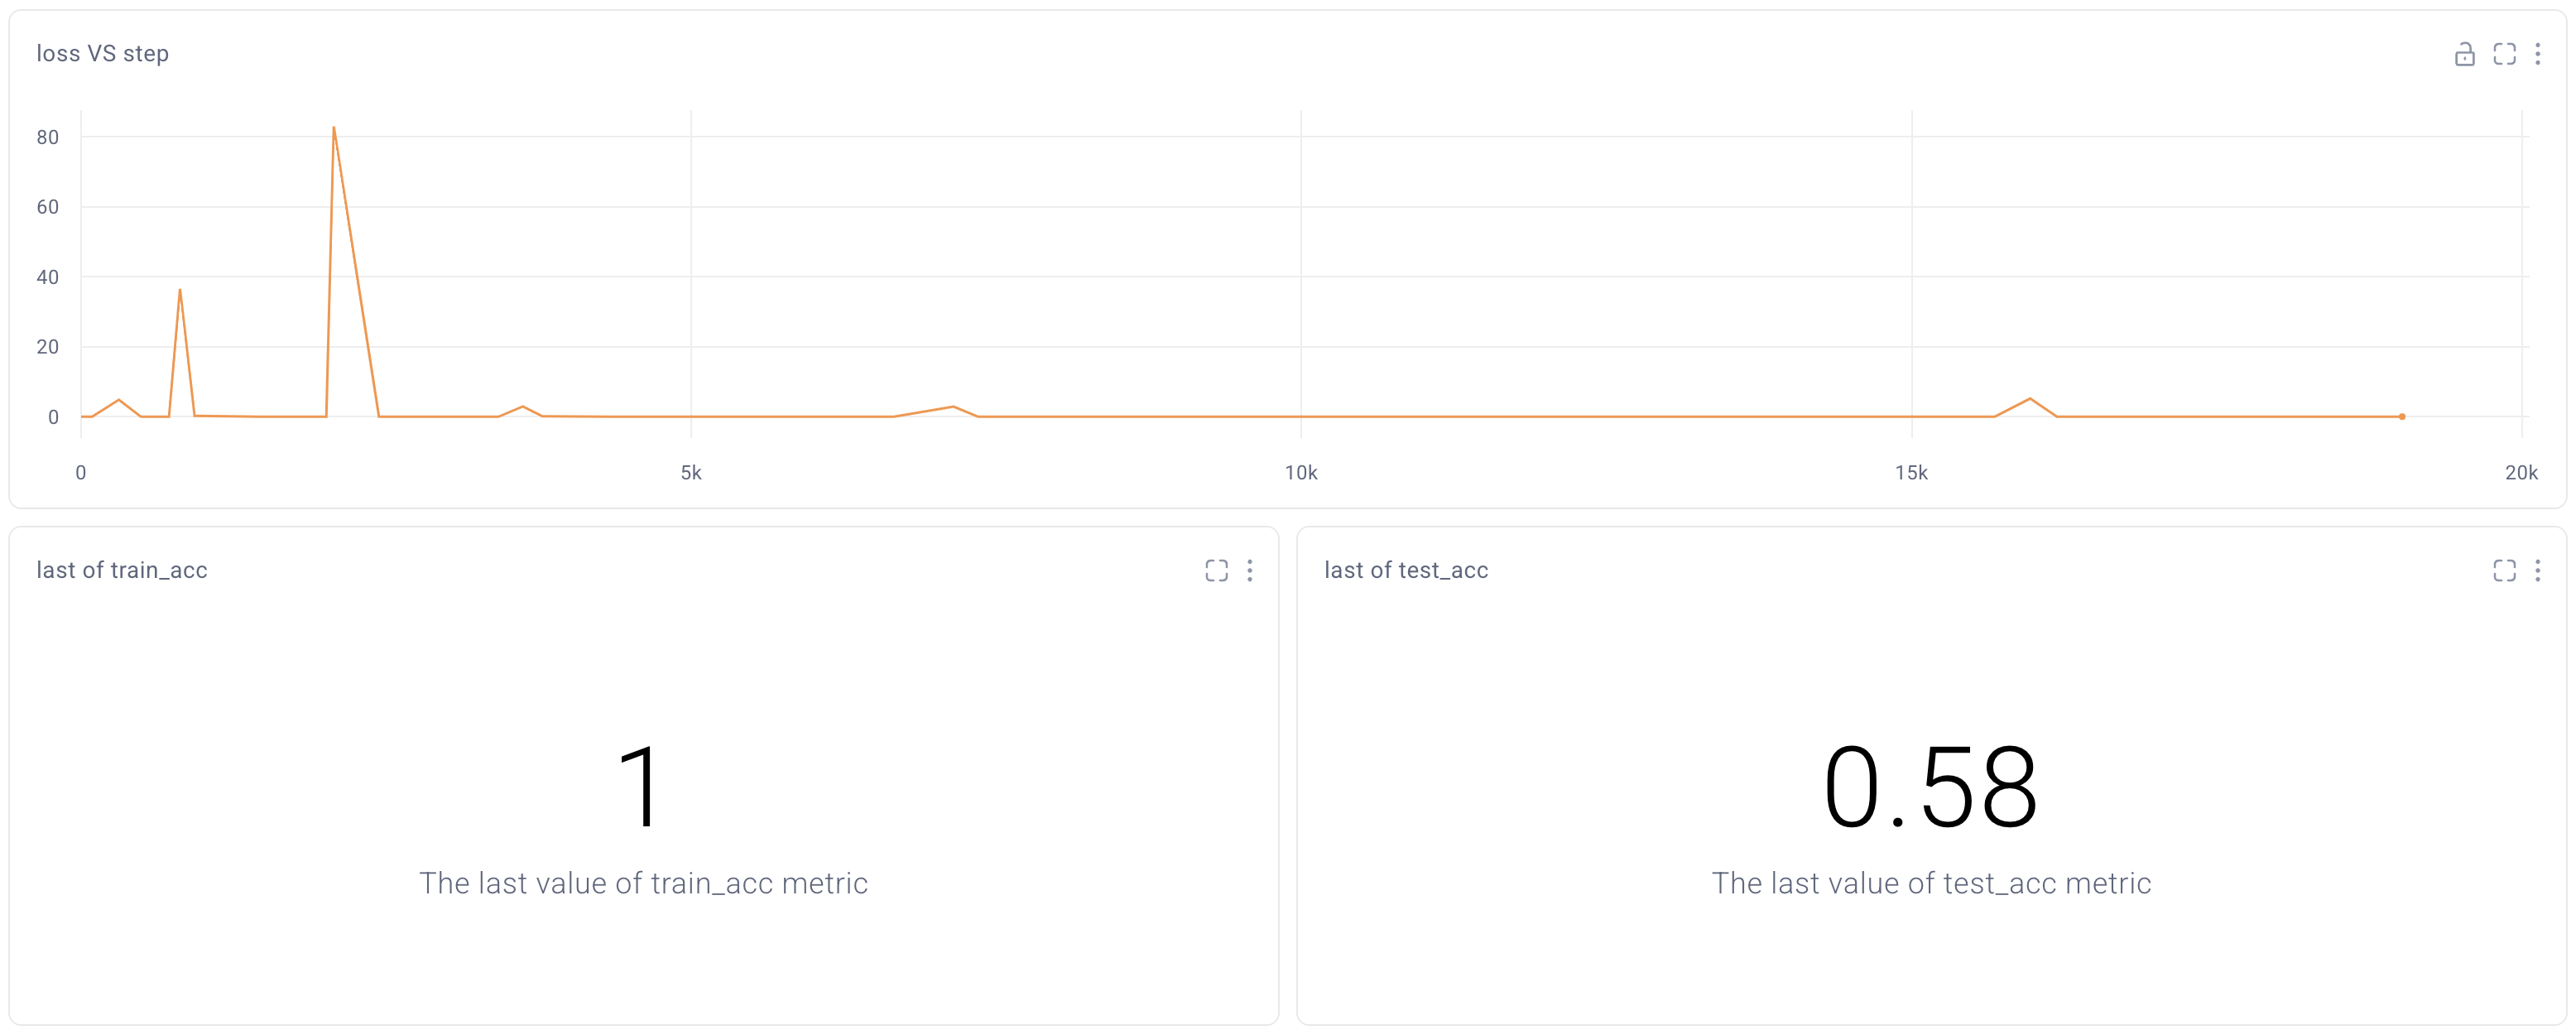
\includegraphics[width=1\textwidth]{figures/fig028.png}
    \caption*{Fonte: Autor}
    \label{fig:fig028}
\end{figure}


\begin{figure}[h!]
    \centering
    \caption{Valores Coletados no Treino - \textit{CometML}}
    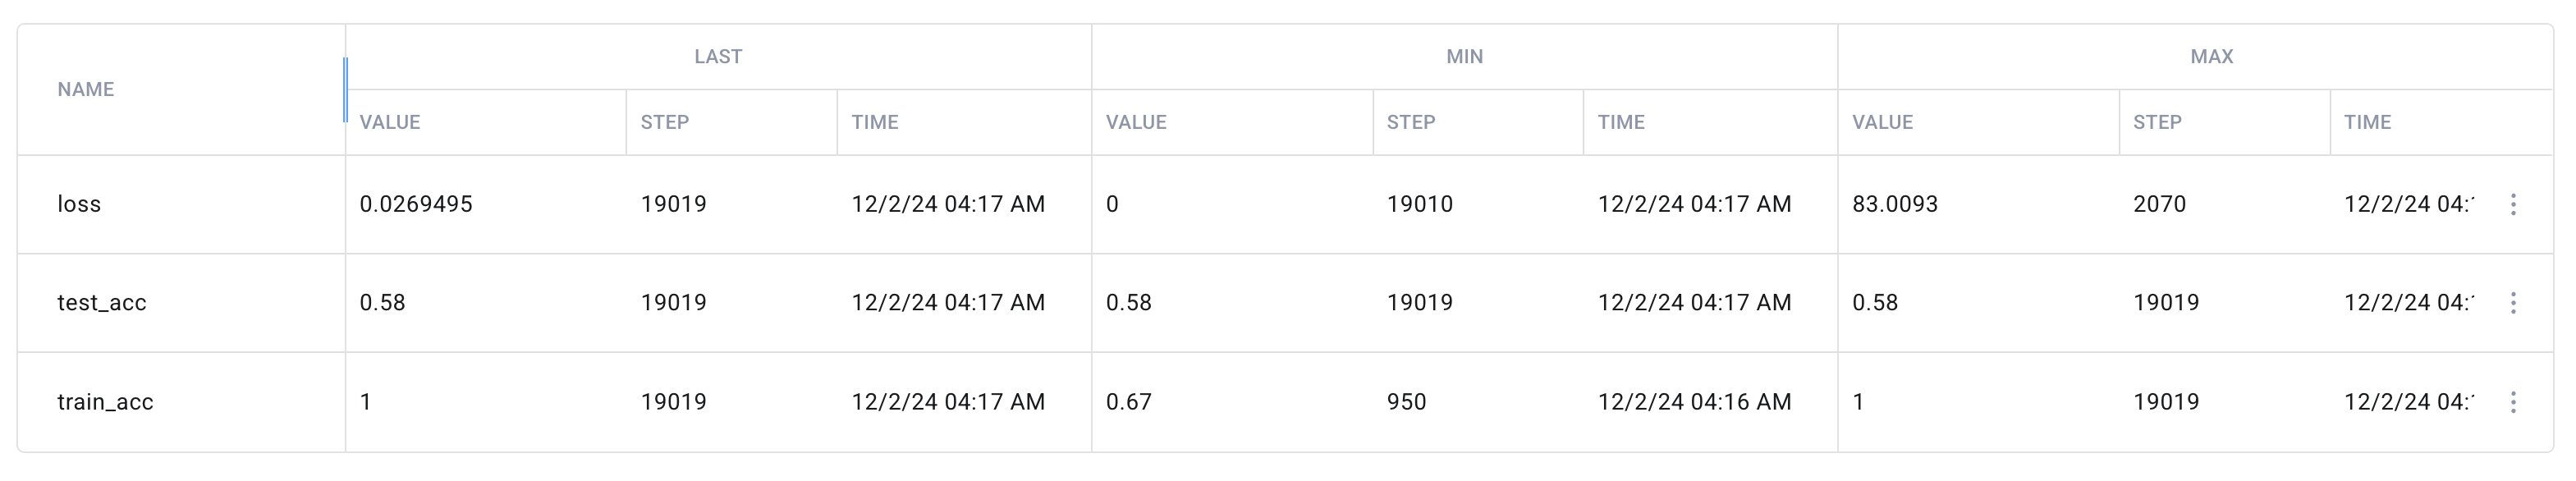
\includegraphics[width=1\textwidth]{figures/fig029.png}
    \caption*{Fonte: Autor}
    \label{fig:fig029}
\end{figure}


%--------------------------------------------------------
\subsection{Resultados dos Modelos Adaptados - ACDC}
\label{subsec:resultados_acdc_adaptado}

Para as versões adaptadas, se buscou mudar os hiperparâmetros e até mesmo a arquitetura do modelo com o intuito comparar os resultados com a versão base. Os primeiros experimentos foram aplicados variando o $\text{EMBED}_{size}$, também foi aplicado $N$ vezes o bloco de autoatenção ao invés de uma única vez. Os experimentos foram executado gerando a combinatória destes hiperparâmetros para cobrir o máximo de cenários possíveis dentro da metodologia.

Também foi introduzido, nas versões adaptadas, um módulo convolucional, que antecede o módulo de autoatenção. Este módulo convolucional é composto de três blocos: uma camada convolucional 1D, um bloco \gls{SE} e outro bloco convolucional 1D. Com a possibilidade de se ter adicionar opcionalmente um terceiro vetor de características, sendo este a máscara, foi possível identificar relações intrínsecas entre mais este vetor. A concatenação agora na primeira dimensão faz cada vetor de característica se tornar um canal. 

No módulo convolucional, uma primeira camada de convolução 1D aumenta o número de canais para $16$, ou seja, $16$ filtros são aplicado para extração de informação espacial. O bloco \gls{SE} representa a camada de atenção seletiva que dá importância aos canais mais importantes, identificando a relevância de cada canal e finaliza escalando os canais na entrada original com um valor escalar otimizado em tempo de treinamento. Detalhes podem ser vistos na Figura \ref{fig:fig031}. O bloco \gls{SE} neste projeto é adaptado para ser 1D, diferente do trabalho original que visa sua aplicação em modelos de visão computacional já consolidados. O valor de $r$ no bloco \gls{SE} ficou fixo em $16$, os autores do trabalho original fazem testes empíricos e confirmam que o valor de $16$ é que traz melhores resultados.

\begin{figure}[h!]
    \centering
    \caption{Composição Bloco SE}
    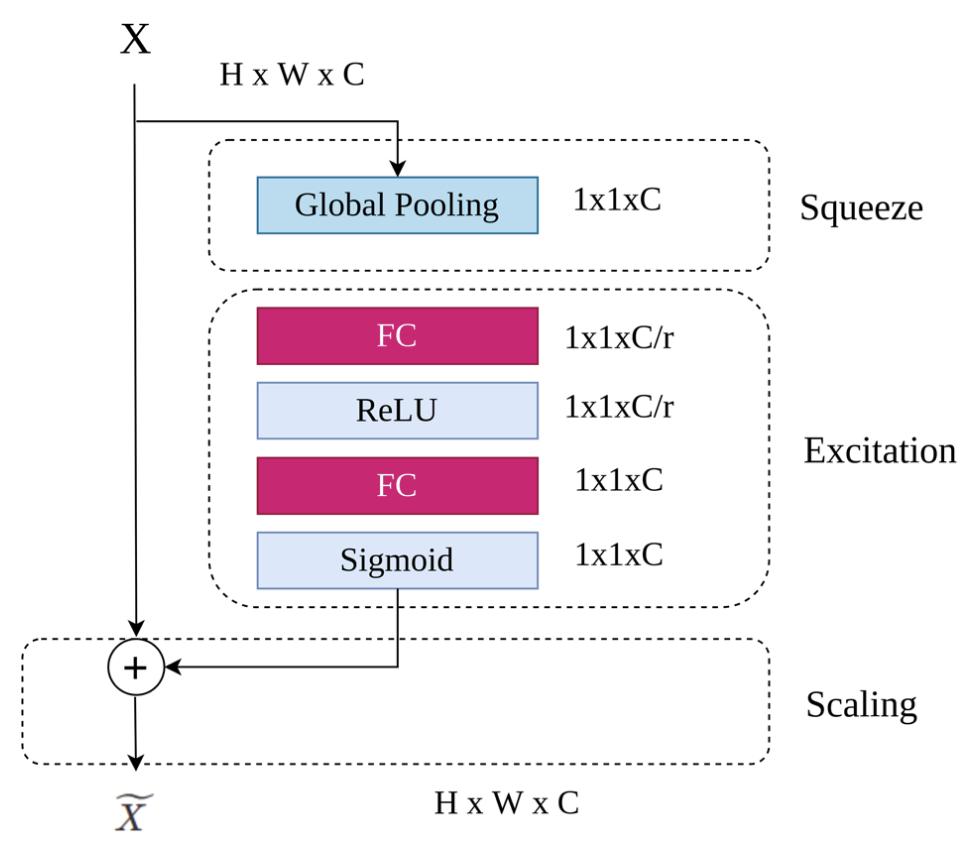
\includegraphics[width=0.7\textwidth]{figures/fig031.png}
    \caption*{Fonte: Adaptado de \cite{lafraxoSEDARUnetSqueezeexcitationDilated2024}}
    \label{fig:fig031}
\end{figure}


A Tabela \ref{tab:metrics_acdc_orig} apresenta o conjunto de experimentos na versão original e versões adaptadas. A Tabela \ref{tab:metrics_acdc_orig_mask} demonstra os experimentos adicionando a máscara como um terceiro vetor de características. A Tabela \ref{tab:metrics_acdc_se} apresenta a adição de blocos convolucionais e  \gls{SE}. Alguns pontos podem ser notados no experimento, o treinamento quase sempre sofre sobre-ajuste ficando muito próximo de 100\% de assertividade, isso pode se justificado dado o fato de haver poucos exemplares para treinamento. Outro ponto notado é que quanto maior o tamanho do vetor de características (Emb) melhor costuma ser o resultado. Quantidades maiores no múmero de blocos de autoatenção (N\_Attn) também melhoram os resultados, exceto no caso em que são configurados em $6$. A justificativa se deve ao fato de tornar o modelo mais complexos se comparados a quantidade de dados para treino, prejudicando a sua capacidade de generalização. Os melhores resultados são conferidos nas versões que adicionam o bloco \gls{SE}, sendo que o melhor experimento obteve $78\%$ de assertividade e aparece em azul. A visualização dos modelos com bloco \gls{SE}, coletados no \textit{CometML} é visto na Figura \ref{fig:fig032}.


\begin{table}[htbp]
\centering
\caption{Métricas ACDC - Adaptação do Modelo Original
\newline Negrito representa o modelo base}
\begin{tabular}{lcccccc}
\toprule
\textbf{Emb} & \textbf{N\_Attn} & \textbf{Acc} & \textbf{Precision} & \textbf{Recall} & \textbf{F1} & \textbf{AUC} \\
\midrule
\textbf{24} & \textbf{1} & \textbf{0.58} & \textbf{0.47} & \textbf{0.45} & \textbf{0.46} & \textbf{0.55} \\
24 & 2 & 0.58 & 0.48 & 0.60 & 0.53 & 0.58 \\
24 & 4 & 0.54 & 0.44 & 0.55 & 0.49 & 0.54 \\
24 & 6 & 0.50 & 0.41 & 0.55 & 0.47 & 0.51 \\
\hline
48 & 1 & 0.62 & 0.52 & 0.55 & 0.54 & 0.61 \\
48 & 2 & 0.64 & 0.54 & 0.65 & 0.59 & 0.64 \\
48 & 4 & 0.66 & 0.56 & 0.70 & 0.62 & 0.67 \\
48 & 6 & 0.64 & 0.54 & 0.70 & 0.61 & 0.65 \\
\hline
64 & 1 & 0.62 & 0.52 & 0.65 & 0.58 & 0.62 \\
64 & 2 & 0.64 & 0.54 & 0.70 & 0.61 & 0.65 \\
64 & 4 & 0.66 & 0.57 & 0.65 & 0.60 & 0.66 \\
64 & 6 & 0.64 & 0.54 & 0.65 & 0.59 & 0.64 \\
\bottomrule
\end{tabular}
\caption*{Fonte: Autor}
\label{tab:metrics_acdc_orig}
\end{table}


\begin{table}[htbp]
\centering
\caption{Métricas ACDC - Adaptação do Modelo Original + Máscaras
\newline Negrito representa maior assertividade}
\begin{tabular}{lcccccc}
\toprule
\textbf{Emb} & \textbf{N\_Attn} & \textbf{Acc} & \textbf{Precision} & \textbf{Recall} & \textbf{F1} & \textbf{AUC} \\
\midrule
24 & 1 & 0.44 & 0.35 & 0.45 & 0.39 & 0.44 \\
24 & 2 & 0.46 & 0.38 & 0.55 & 0.45 & 0.48 \\
24 & 4 & 0.48 & 0.36 & 0.40 & 0.38 & 0.47 \\
24 & 6 & 0.48 & 0.38 & 0.45 & 0.41 & 0.47 \\
\hline
48 & 1 & 0.52 & 0.44 & 0.70 & 0.54 & 0.55 \\
48 & 2 & 0.58 & 0.48 & 0.55 & 0.51 & 0.57 \\
48 & 4 & 0.62 & 0.52 & 0.60 & 0.56 & 0.62 \\
48 & 6 & 0.60 & 0.50 & 0.50 & 0.50 & 0.58 \\
\hline
64 & 1 & 0.58 & 0.48 & 0.60 & 0.53 & 0.58 \\
64 & 2 & 0.56 & 0.45 & 0.50 & 0.48 & 0.55 \\
\textbf{64} & \textbf{4} & \textbf{0.64} & \textbf{0.54} & \textbf{0.65} & \textbf{0.59} & \textbf{0.64} \\
64 & 6 & 0.62 & 0.53 & 0.45 & 0.49 & 0.59 \\
\bottomrule
\end{tabular}
\caption*{Fonte: Autor}
\label{tab:metrics_acdc_orig_mask}
\end{table}


\begin{table}[htbp]
\centering
\caption{Métricas ACDC - Modelos Adaptados - Blocos Conv. + SE
\newline Negrito representa maior assertividade}
\begin{tabular}{lcccccc}
\toprule
\textbf{Emb} & \textbf{N\_Attn} & \textbf{Acc} & \textbf{Precision} & \textbf{Recall} & \textbf{F1} & \textbf{AUC} \\
\midrule
24 & 1 & 0.66 & 0.56 & 0.70 & 0.62 & 0.67 \\
24 & 2 & 0.68 & 0.58 & 0.75 & 0.65 & 0.69 \\
24 & 4 & 0.70 & 0.59 & 0.80 & 0.68 & 0.72 \\
24 & 6 & 0.68 & 0.59 & 0.65 & 0.62 & 0.67 \\
\hline
48 & 1 & 0.70 & 0.58 & 0.90 & 0.71 & 0.73 \\
48 & 2 & 0.70 & 0.62 & 0.65 & 0.63 & 0.69 \\
48 & 4 & 0.74 & 0.65 & 0.75 & 0.70 & 0.74 \\
48 & 6 & 0.70 & 0.60 & 0.75 & 0.67 & 0.71 \\
\hline
64 & 1 & 0.64 & 0.54 & 0.65 & 0.59 & 0.64 \\
64 & 2 & 0.72 & 0.64 & 0.70 & 0.67 & 0.72 \\
\textbf{64} & \textbf{4} & \textbf{0.78} & \textbf{0.76} & \textbf{0.65} & \textbf{0.70} & \textbf{0.76} \\
64 & 6 & 0.76 & 0.65 & 0.85 & 0.74 & 0.77 \\
\bottomrule
\end{tabular}
\caption*{Fonte: Autor}
\label{tab:metrics_acdc_se}
\end{table}


\begin{figure}[h!]
    \centering
    \caption{Modelos c/ Bloco SE e sua Acurácia - \textit{CometML}}
    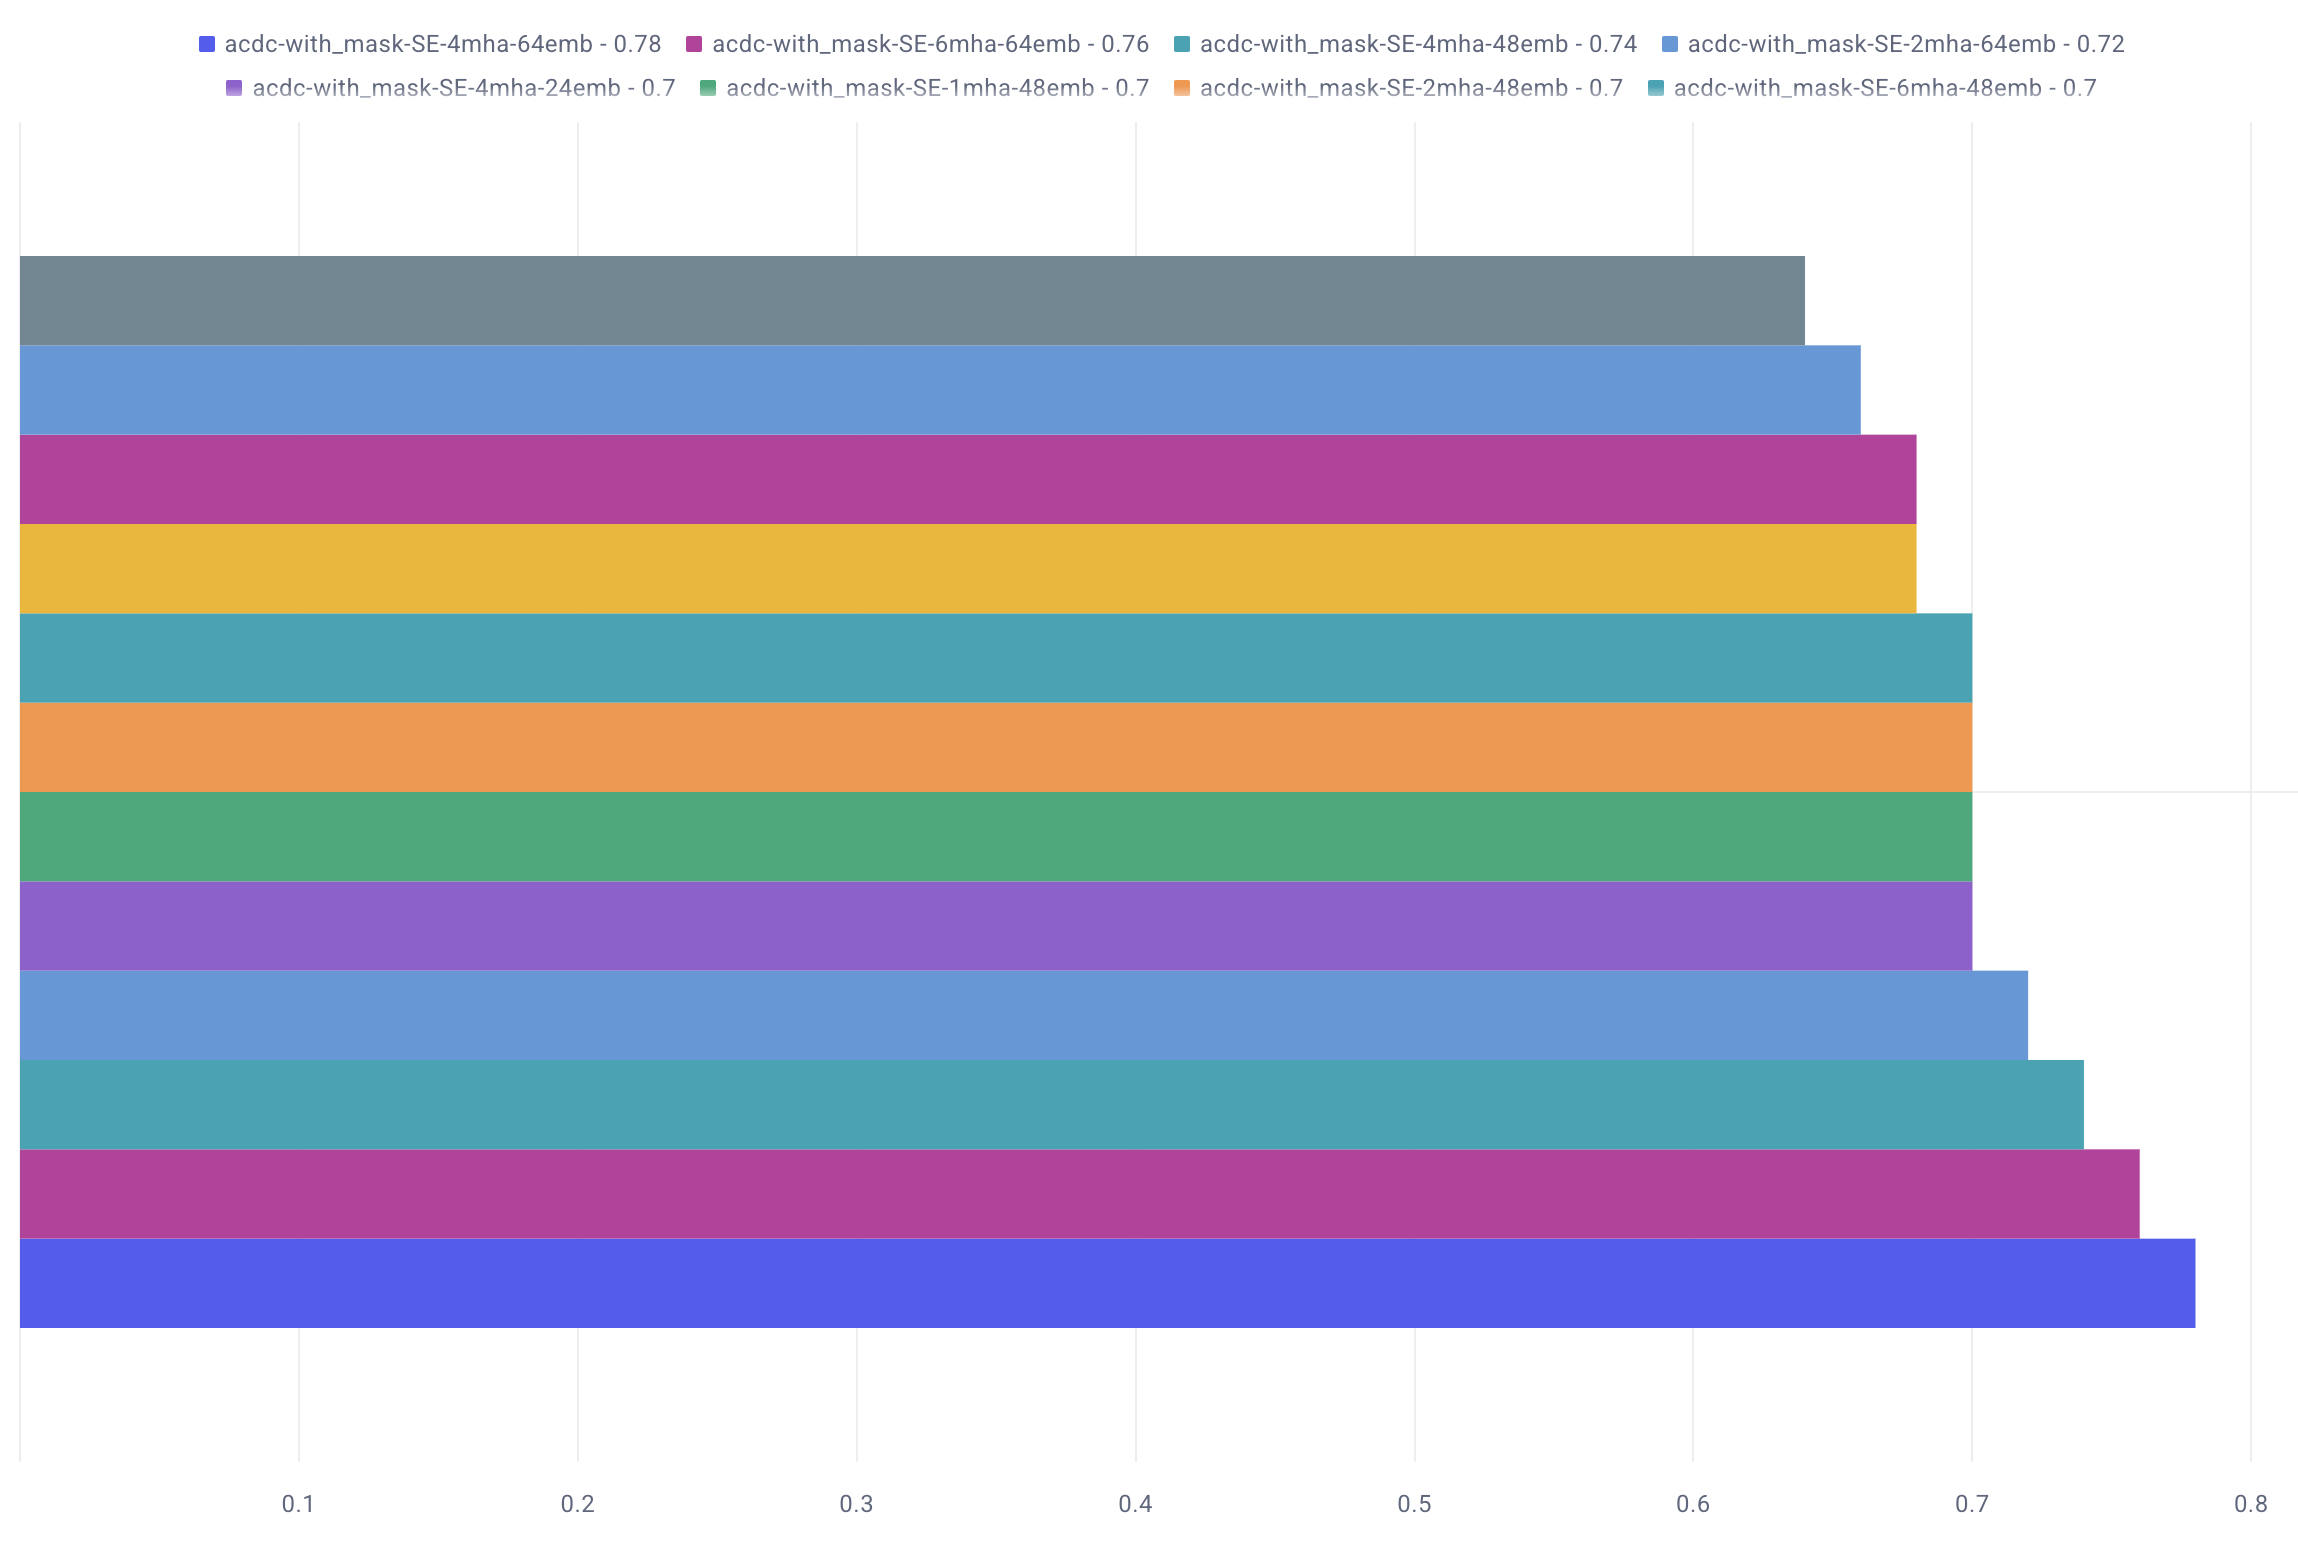
\includegraphics[width=1\textwidth]{figures/fig032.png}
    \caption*{Fonte: Autor}
    \label{fig:fig032}
\end{figure}

%--------------------------------------------------------
\subsection{Resultados dos Modelos Adaptados - \textit{SunnyBrook}}
\label{subsec:resultados_sunny_adaptado}

Os experimentos no conjunto de dados \textit{SunnyBrook} foram os mesmos aplicados ao conjunto de dados \gls{ACDC}. No conjunto de dados \textit{SunnyBrook}, houve uma etapa extra de pré-processamento para gerar as máscaras. Foi necessário interpolar os valores de um arquivo de texto que vem anexo com os dados. A máscara também é composta apenas pela região de interesse com valores entre 0 e 1.

Como o \textit{SunnyBrook} tem poucos dados, apenas $45$, sendo $30$ para treino e $15$ para teste e removendo as classes de infarto (IC e IC-I), sobram $21$ registros sendo $13$ para treino e $8$ para teste. Foi considerado que o treinamento neste conjunto de dados não seria benéfico, pela quantidade limitada. Foi aplicado apenas as inferências considerando os $21$ registros, sendo $12$ casos de \gls{CMH} e $9$ casos em condições normais. Os modelos utilizados são os previamente treinados no \gls{ACDC}. Os resultados são conferidos nas tabelas \ref{tab:metrics_sunny_orig}, \ref{tab:metrics_sunny_orig_mask} e \ref{tab:metrics_sunny_se}. O modelo base consta em laranja e o melhor resultado consta em azul, indo de encontro aos resultados obtidos no \gls{ACDC}. É possível notar que o conjunto de dados, por ser pequeno, compromete a classificação pois mesmo que o modelo possua um pequeno aprimoramento de uma arquitetura para outra, pode não ser suficiente para converter uma nova classificação, o que da a aparência de que alguns modelos possuem a mesma capacidade, o que não é a realidade.


\begin{table}[htbp]
\centering
\caption{Métricas SunnyBrook - Adaptação do Modelo Original
\newline Negrito representa o modelo base}
\begin{tabular}{ccccccc}
\toprule
\textbf{Emb} & \textbf{N\_Attn} & \textbf{Acc} & \textbf{Precision} & \textbf{Recall} & \textbf{F1} & \textbf{AUC} \\
\midrule
\textbf{24} & \textbf{1} & \textbf{0.48} & \textbf{0.54} & \textbf{0.58} & \textbf{0.56} & \textbf{0.46} \\
24 & 2 & 0.52 & 0.60 & 0.50 & 0.55 & 0.53 \\
24 & 4 & 0.52 & 0.60 & 0.50 & 0.55 & 0.53 \\
24 & 6 & 0.52 & 0.57 & 0.67 & 0.62 & 0.50 \\
48 & 1 & 0.48 & 0.56 & 0.42 & 0.48 & 0.49 \\
48 & 2 & 0.48 & 0.55 & 0.50 & 0.52 & 0.47 \\
48 & 4 & 0.52 & 0.58 & 0.58 & 0.58 & 0.51 \\
48 & 6 & 0.52 & 0.60 & 0.50 & 0.55 & 0.53 \\
64 & 1 & 0.52 & 0.57 & 0.67 & 0.62 & 0.50 \\
64 & 2 & 0.57 & 0.64 & 0.58 & 0.61 & 0.57 \\
64 & 4 & 0.57 & 0.67 & 0.50 & 0.57 & 0.58 \\
64 & 6 & 0.52 & 0.57 & 0.67 & 0.62 & 0.50 \\
\bottomrule
\end{tabular}
\caption*{Fonte: Autor}
\label{tab:metrics_sunny_orig}
\end{table}


\begin{table}[htbp]
\centering
\caption{Métricas SunnyBrook - Adaptação do Modelo Original Com Máscaras
\newline Negrito representa maior assertividade}
\begin{tabular}{ccccccc}
\toprule
\textbf{Emb} & \textbf{N\_Attn} & \textbf{Acc} & \textbf{Precision} & \textbf{Recall} & \textbf{F1} & \textbf{AUC} \\
\midrule
24 & 1 & 0.48 & 0.54 & 0.58 & 0.56 & 0.46 \\
24 & 2 & 0.52 & 0.62 & 0.42 & 0.50 & 0.54 \\
24 & 4 & 0.57 & 0.67 & 0.50 & 0.57 & 0.58 \\
24 & 6 & 0.52 & 0.58 & 0.58 & 0.58 & 0.51 \\
48 & 1 & 0.52 & 0.58 & 0.58 & 0.58 & 0.51 \\
48 & 2 & 0.57 & 0.64 & 0.58 & 0.61 & 0.57 \\
48 & 4 & 0.62 & 0.67 & 0.67 & 0.67 & 0.61 \\
48 & 6 & 0.52 & 0.58 & 0.58 & 0.58 & 0.51 \\
64 & 1 & 0.57 & 0.62 & 0.67 & 0.64 & 0.56 \\
64 & 2 & 0.62 & 0.67 & 0.67 & 0.67 & 0.61 \\
\textbf{64} & \textbf{4} & \textbf{0.71} & \textbf{0.80} & \textbf{0.67} & \textbf{0.73} & \textbf{0.72} \\
64 & 6 & 0.62 & 0.64 & 0.75 & 0.69 & 0.60 \\
\bottomrule
\end{tabular}
\caption*{Fonte: Autor}
\label{tab:metrics_sunny_orig_mask}
\end{table}


\begin{table}[htbp]
\centering
\caption{Métricas SunnyBrook - Adaptação Adicionando Blocos Conv. e SE
\newline Negrito representa maior assertividade}
\begin{tabular}{ccccccc}
\toprule
\textbf{Emb} & \textbf{N\_Attn} & \textbf{Acc} & \textbf{Precision} & \textbf{Recall} & \textbf{F1} & \textbf{AUC} \\
\midrule
24 & 1 & 0.67 & 0.73 & 0.67 & 0.70 & 0.67 \\
24 & 2 & 0.71 & 0.80 & 0.67 & 0.73 & 0.72 \\
24 & 4 & 0.76 & 0.77 & 0.83 & 0.80 & 0.75 \\
24 & 6 & 0.71 & 0.75 & 0.75 & 0.75 & 0.71 \\
48 & 1 & 0.71 & 0.80 & 0.67 & 0.73 & 0.72 \\
48 & 2 & 0.76 & 0.82 & 0.75 & 0.78 & 0.76 \\
48 & 4 & 0.76 & 0.73 & 0.92 & 0.81 & 0.74 \\
48 & 6 & 0.76 & 0.89 & 0.67 & 0.76 & 0.78 \\
64 & 1 & 0.76 & 0.82 & 0.75 & 0.78 & 0.76 \\
64 & 2 & 0.81 & 0.90 & 0.75 & 0.82 & 0.82 \\
\textbf{64} & \textbf{4} & \textbf{0.86} & \textbf{0.85} & \textbf{0.92} & \textbf{0.88} & \textbf{0.85} \\
64 & 6 & 0.81 & 0.90 & 0.75 & 0.82 & 0.82 \\
\bottomrule
\end{tabular}
\caption*{Fonte: Autor}
\label{tab:metrics_sunny_se}
\end{table}

%--------------------------------------------------------
\section{Considerações Finais do Capítulo} 
\label{sec:cap6_consideracoes_finais}

Os resultados obtidos, aplicando a arquitetura original proposta por \citeonline{aiSelfAttentionBasedFusion2023} e a aplicação de diversas modificações, como a forma de concatenar para propiciar um módulo convolucional de extrair informações inter-relacionadas entre características extraídas de diferentes técnicas, a adição de um mecanismo de atenção seletiva na forma de um bloco \gls{SE} antecedente ao mecanismo de autoatenção, seguiram um padrão de resultados esperados. Conforme o modelo aumenta, seus resultados também melhoram mas com ganhos mínimos dependendo do caso. Adicionar técnicas relevantes como o bloco \gls{SE} aprimorou os resultados significativamente.

A atenção seletiva procura gera um conjunto de pesos ao ao prever diretamente a importância de cada parte dos dados, aprendendo o valor dos pesos para cada canal no mapa de características com o objetivo de realçar ou suprimir as características de cada canal. O mecanismo de autoatenção envolve a utilização da correlação entre os conteúdos das camadas ocultas para calcular os pesos de atenção, que são então aplicados para agregar informações das camadas ocultas em uma escala global. Seguindo a intuição de utilizar diferentes mecanismos de atenção, conforme proposto pelos autores \cite{yangNeuralNetworkDesign2024a}, trouxe melhoras significativas comparadas ao modelo base. 

Outras adaptações também surtiram efeito, como aumentar o tamanho das características utilizadas, aplicar mais blocos de autoatenção, a adição das máscaras, etc. Os experimentos indicam que há espaço para exploração e melhorias, como por exemplo, outros mecanismos de atenção, podem trazer resultados ainda mais promissores para o âmbito de cardiomiopatia hipertrófica. 

